\input{head.inc}

% Präambelbefehle für die Präsentation
\title[TET: Verhalten an Grenzflächen]{Verhalten an Grenzflächen}

\begin{document}
% 
% Frontmatter 
% 
%%%%%%%%%%%%%%%%%%%%%%%%%%%%%%%%%%%%%%%%%%%%%%%%%%%%%%%%%%%%%%%%%%%%%%%%%%%%%%%%%%%%%%%%%%%%%%%%%%%%%%%%%%%%%%%%%%%%%%%%%%%%% 

%% inserts the title page and the table of contents
\maketitle

% 
% Content 
% 
%%%%%%%%%%%%%%%%%%%%%%%%%%%%%%%%%%%%%%%%%%%%%%%%%%%%%%%%%%%%%%%%%%%%%%%%%%%%%%%%%%%%%%%%%%%%%%%%%%%%%%%%%%%%%%%%%%%%%%%%%%%%% 
\section{Verhalten an Grenzflächen}

\begin{frame}
  \frametitle{Normalkomponenten von $\vec{D}$ und $\vec{B}$}
\begin{columns}
  \begin{column}{0.4\textwidth}
    Gaußsche Dose:\\[2em]

    
	\resizebox{\columnwidth}{!}{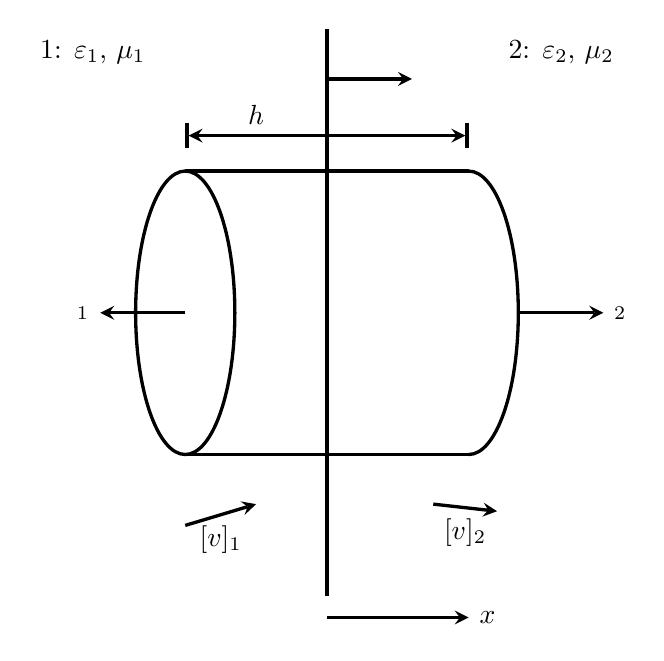
\begin{tikzpicture}[line width = 1.2pt, line join=round,x=1cm,y=1cm,>=stealth, scale = 0.9]
	% Medien und ihre Kennwerte
	\draw (-4.2,4) node [anchor=north west] {\circled{1}: $ \varepsilon_1 $, $ \mu_1$};
	\draw (4.2,4) node [anchor = north east] {\circled{2}: $ \varepsilon_2 $, $ \mu_2$};
	% linke Grundfläche
	\draw (-2,0) ellipse (0.7 and 2);
	% Beschriftung der Grundfläche
	\draw (-2,0.5) node [anchor=south] {$ \Flaeche{} $};
	\draw (-2,-0.5) node [anchor = north] {$ \volumen $};
	% rechte Grundfläche
	\draw (2.7,0) arc (0:90:0.7 and 2);
	\draw (2.7,0) arc (0:-90:0.7 and 2);
	% Mittelachse
	\draw (0,4) -- (0,-4);
	% obere und untere Begrenzung
	\draw (-2,2) -- (2,2);
	\draw (-2,-2) -- (2,-2);
	% Verschiebungsvektoren
	\draw[->] (-2,-3) -- (-1,-2.7) node [midway, below] {$ \DFeld[v]_1 $};
	\draw[->] (1.5,-2.7) -- (2.4,-2.8) node [midway, below] {$ \DFeld[v]_2 $};
	% x-Richtung
	\draw [->] (0,-4.3) -- (2,-4.3) node [anchor = west] {$ x $};
	% die Normalen
	\draw [->] (0,3.3) -- (1.2,3.3) node [anchor= west] {$ \normalenvektor $};
	\draw [->] (-2,0) -- (-3.2,0) node [anchor = east] {$ \normalenvektor_1 $};
	\draw [->] (2.7,0) -- (3.9,0) node [anchor = west] {$ \normalenvektor_2 $};
	% Höhe
	\draw [|<->|] (-2,2.5) -- (2,2.5) node [near start, above] {$ h $};
\end{tikzpicture}}

    \end{column}
    \begin{column}{0.6\textwidth}
      \begin{itemize}
        \item<1-> Coulomb-Gauß-Gesetz: $\divergenz \verschiebung[v] =
          \laddichte{V}$
          \item<2-> Volumenintegral: \only<2>{$\iiint\limits_{\volumen}
              \divergenz \verschiebung[v] \intvolumen =
              \iiint\limits_{\volumen} \laddichte{V} \intvolumen$}
            \only<3->{$\oiint\limits_{\oberfl(\volumen)}
              \verschiebung[v] \cdot \intflaeche[v] =
              \iiint\limits_{\volumen} \laddichte{V} \intvolumen$}
          \item<4-> Grenzübergang $h\to0$
            \item<5-> \only<5>{$\left( \vec{n}_1\cdot \vec{D}_1 +
                \vec{n}_2\cdot \vec{D}_2\right) A =
              \iiint\limits_{\volumen} \laddichte{F} \cdot \delta(x)
              \intvolumen = \laddichte{F} \cdot \flaeche$}
            \only<6->{$\left( - \vec{n}\cdot \vec{D}_1 +
                \vec{n}\cdot \vec{D}_2\right) A =
              \iiint\limits_{\volumen} \laddichte{F} \cdot \delta(x)
              \intvolumen = \laddichte{F} \cdot \flaeche$}
          \item<7-> \alert{Normalkomponente von $\vec{D}$ ist ggf. unstetig:} 
            $$	\boxed{\verschiebung{}_2\normal -
              \verschiebung{}_1\normal = \laddichte{F}} $$
          \item<8-> Analog aus $\divergenz \tetB[v] = 0$
            \item<9-> \alert{Normalkomponente von $\vec{B}$ ist immer stetig:} 
            $$		\boxed{\tetB{}_2\normal - \tetB{}_1\normal = 0} $$
        \end{itemize}
    \end{column}
\end{columns}
 \end{frame}

 \begin{frame}
  \frametitle{Tangentialkomponenten von $\vec{E}$ und $\vec{H}$}
\begin{columns}
  \begin{column}{0.4\textwidth}
    Stokesche Fläche:\\[2em]

    
	\resizebox{.7\columnwidth}{!}{\begin{tikzpicture}[line width = 1.2pt, line join=round,x=0.5cm,y=0.5cm,>=stealth]
	% Mittellinie zeichnen
	\draw (0,-6) -- (0,7);
	% Schleife zeichnen
	\draw (-1.5,-5) rectangle (1.5,5);
	% Richtungen der Schleife
	\draw [->] (-1.5,3) -- (-1.5,2);
	\draw [->] (1.5,1) -- (1.5,2);
	% Vektoren für ds Zeichnen
	\draw [->,line width = 2pt] (-1.5,0) -- (-1.5,-2);
	\draw (-1.5,-1) node[anchor=east] {$\upd \weg[v]_1$};
	\draw [->,line width = 2pt] (1.5,-2) -- (1.5,0);
	\draw (1.5,-1) node[anchor=west] {$\upd \weg[v]_2$};
	% Breite der Schleife
	\draw [|<->|] (1.5,5.5) -- (-1.5,5.5) node[anchor=south west] {$ h $};
	% Höhe der Schleife
	\draw [|<->|] (-3.5,-5) -- (-3.5,5);
	\draw (-3.5,0) node[anchor=east] {$ l $};
	% Normalenvektor
	\draw [->] (0,6.5) -- (2,6.5) node[anchor=west] {$ \normalenvektor $};
	% Tangentialvektor
	\draw [->] (0,6.5) -- (0,8.5) node[anchor=south] {$ \tangentialvektor $};
	% Flächenbezeichnung und Randbezeichnung
	\draw (0,-4.3) node[anchor=west] {$ \flaeche $};
	\draw (1.5,-4.3) node[anchor=west] {$ \rand(\flaeche) $};
	% elektrisches Feld
	\draw [->] (-2.5,-6) -- (-1,-5.6) node[anchor=north east] {$ \efeld[v]_1 $};
	\draw [->] (1,-5.9) -- (2.55,-5.7) node[anchor=north east] {$ \efeld[v]_2 $};
	% Definition der Seiten
	\draw (-4,8) node[anchor=west] {\circled{1}};
	\draw (4,8) node[anchor=east] {\circled{2}};
\end{tikzpicture}}

    \end{column}
    \begin{column}{0.6\textwidth}
      \begin{itemize}
        \item<1-> Induktionsgesetz: $	\rotation \efeld[v] = -\dfrac{\partial \tetB[v]}{\partial t}$
          \item<2-> Flächenintegral: \only<2>{$\iint\limits_{\flaeche} \rotation \efeld[v]\cdot \intflaeche[v] = -\iint\limits_{\flaeche} \dfrac{\partial \tetB[v]}{\partial t}\cdot \intflaeche[v]$}
            \only<3->{$\oint\limits_{\rand(A)}  \efeld[v] \cdot\intweg[v] = -\iint_{\flaeche} \dfrac{\partial \tetB[v]}{\partial t} \cdot\intflaeche[v]$}
          \item<4-> Grenzübergang $h\to0$, Flußänderung verschwindet
            \item<5-> $-\efeld{}_1\tangential \cdot l + \efeld{}_2\tangential \cdot l = 0$
          \item<6-> \alert{Tangentialkomponente von $\vec{E}$ ist immer stetig:} 
            $$		\boxed{\efeld{}_2\tangential - \efeld{}_1\tangential = 0} $$
          \item<7-> Der Tangentialvektor $\tangentialvektor$ ist nicht
            eindeutig. Die Beziehung gilt für alle möglichen
            Tangentialvektoren $	\tangentialvektor \bot \normalenvektor $
        \end{itemize}
    \end{column}
\end{columns}
 \end{frame}

 \begin{frame}
  \frametitle{Tangentialkomponenten von $\vec{E}$ und $\vec{H}$}
\begin{columns}
  \begin{column}{0.4\textwidth}
 	\resizebox{.7\columnwidth}{!}{\begin{tikzpicture}[line width = 1.2pt, line join=round,x=0.5cm,y=0.5cm,>=stealth]
	% Mittellinie zeichnen
	\draw (0,-6) -- (0,7);
	% Schleife zeichnen
	\draw (-1.5,-5) rectangle (1.5,5);
	% Richtungen der Schleife
	\draw [->] (-1.5,3) -- (-1.5,2);
	\draw [->] (1.5,1) -- (1.5,2);
	% Vektoren für ds Zeichnen
	\draw [->,line width = 2pt] (-1.5,0) -- (-1.5,-2);
	\draw (-1.5,-1) node[anchor=east] {$\upd \weg[v]_1$};
	\draw [->,line width = 2pt] (1.5,-2) -- (1.5,0);
	\draw (1.5,-1) node[anchor=west] {$\upd \weg[v]_2$};
	% Breite der Schleife
	\draw [|<->|] (1.5,5.5) -- (-1.5,5.5) node[anchor=south west] {$ h $};
	% Höhe der Schleife
	\draw [|<->|] (-3.5,-5) -- (-3.5,5);
	\draw (-3.5,0) node[anchor=east] {$ l $};
	% Normalenvektor
	\draw [->] (0.3,-10) -- (2,-10) node[anchor=west] {$ \normalenvektor $};
	% Tangentialvektor
	\draw [->] (0,-9.7) -- (0,-8) node[anchor=south] {$ \tangentialvektor $};
	% Tangentialvektor 2
	\draw (0,-10) circle (0.3);
	\filldraw (0,-10) circle (1.2pt);
	\draw (0,-10.3) node[anchor=north] {$ \tangentialvektor_2 $};
	% Flächenbezeichnung und Randbezeichnung
	\draw (0,-4.3) node[anchor=west] {$ \flaeche $};
	\draw (1.5,-4.3) node[anchor=west] {$ \rand(\flaeche) $};
	% magnetisches Feld
	\draw [->] (-2.5,-6) -- (-1,-5.6) node[anchor=north east] {$ \magfeld[v]_1 $};
	\draw [->] (1,-5.9) -- (2.55,-5.7) node[anchor=north east] {$ \magfeld[v]_2 $};
	% Definition der Seiten
	\draw (-4,7.5) node[anchor=west] {\circled{1}};
	\draw (4,7.5) node[anchor=east] {\circled{2}};
\end{tikzpicture}}

    \end{column}
    \begin{column}{0.6\textwidth}
      \begin{itemize}[<+->]
        \item Durchflutungsgesetz: $	\rotation \magfeld[v] = \elstromdichte[v] + \dfrac{\partial \verschiebung[v]}{\partial t}$
          \item Flächenintegral, $h\to 0$, Änderung Verschiebungsstrom
            = 0:
            $$-\magfeld_1\tangential \cdot l +
              \magfeld_2\tangential \cdot l = \iint\limits_{\flaeche} \elstromdichte[v]\cdot \intflaeche[v] = \iint\limits_{\flaeche} \elstromdichte[v]_\mathrm{\flaeche}  \delta(x) \cdot\intflaeche[v] = \elstromdichte{}_\mathrm{\flaeche}\tangential[2] \cdot l$$
          \item \alert{Tangentialkomponente von $\vec{H}$ ist ggf. unstetig:} 
            $$			\boxed{\magfeld_2\tangential - \magfeld_1\tangential = \elstromdichte{}_\mathrm{\flaeche}\tangential[2]} $$
          \item Die Beziehung gilt für alle möglichen
            Tangentialvektoren mit $\tangentialvektor_2 = \normalenvektor \times \tangentialvektor $
        \end{itemize}
    \end{column}
\end{columns}
 \end{frame}
\input{finalframe.inc}
\end{document}